% =======================================================================================
\section{The Gravitational-Wave Problem}
\label{sec:gw}
% =======================================================================================
% Moved 2026-11-09 from the former sections/problem.tex (data, prior) and the data tokens of the
% former Network subsection; subsections in the order priors, rates, waveforms, frequency-domain
% factorisation, slicing in frequency, tokenisation. 2026-11-10: the equations, tab:priors-source,
% fig:priors and fig:noise-psd of 4.1-4.3 were MOVED here from app:priors, app:forward-model and
% app:noise (labels unchanged; the appendices now refer to them). Still in the appendices: why the band
% can be sliced (app:forward-model-windows), the bands and their response lengths (tab:forward-model-bands).

A \ac{gb} is a circular, slowly chirping binary. Its signal is fixed by eight
parameters $\theta=(f_0,\fdot,\Amp,\alpha,\delta,\psi,\iota,\phi_0)$: frequency, frequency
derivative, amplitude, sky position, polarisation, inclination and initial phase
(\cref{app:forward-model}).

\subsection{Priors}
\label{sec:gw-priors}
% Equations, table and figure moved 2026-11-10 from app:priors (the details stay there).

Given the window centre $\fw$, a window's $S$ sources, $S$ fixed per run, are independent draws
from one per-source prior $\pi_w(\theta) = \pi(\theta\mid\fw)$ (\cref{tab:priors-source}),
\begin{equation}
  \pi_w(\theta_{1:S}) = \prod_{s=1}^{S}\pi_w(\theta_s).
  \label{eq:priors-window-prior}
\end{equation}
Frequency, drift and amplitude follow one Gaussian in their logarithms, the maximum-likelihood fit
to the double white dwarfs above \qty{\PriorsCatalogueCutMhz}{\milli\hertz} of a simulated Galactic
catalogue \citep{lamberts2019predicting,toubiana2024interacting,perego2025towards,breivik2020cosmic}
\textcolor{red}{TODO(confirm): the catalogue's own reference, \cref{app:priors-sources}},
\begin{equation}
  \begin{pmatrix}\log_{10}f_0\\ \log_{10}\fdot\\ \log_{10}\Amp\end{pmatrix}
  \sim \Normal(\mu, \Sigma),\qquad
  \mu = \begin{pmatrix}\PriorsMeanF\\ \PriorsMeanFdot\\ \PriorsMeanAmp\end{pmatrix},
  \label{eq:priors-source}
\end{equation}
with $f_0$ in \unit{\hertz}, $\fdot$ in \unit{\hertz\per\second}, the covariance $\Sigma$ in
\cref{app:priors-sources}, and $f_0$ truncated to the window (\cref{eq:priors-interior}). Given
$f_0$, the drift and amplitude are Gaussian with means linear in $\log_{10}f_0$,
\begin{equation}
\begin{aligned}
  \log_{10}\fdot \mid f_0 &\sim \Normal\bigl(\PriorsInterceptFdot + \PriorsSlopeFdot\log_{10}f_0,\ \PriorsResidualFdot^2\bigr),\\
  \log_{10}\Amp \mid f_0 &\sim \Normal\bigl(\PriorsInterceptAmp + \PriorsSlopeAmp\log_{10}f_0,\ \PriorsResidualAmp^2\bigr),
\end{aligned}
  \label{eq:priors-conditional}
\end{equation}
the drift's slope close to the $11/3$ of a chirp driven by radiation reaction
(\cref{eq:forward-model-fdot}). Population models of the Galaxy's double white dwarfs
\citep{nelemans2001gravitational,toonen2012supernova,korol2017prospects,korol2020populations,georgousi2022gravitational,thiele2023applying}
differ in their binary physics
\citep{biscoveanu2023probing,toubiana2024interacting,boileau2025gravitational,delfavero2025recovering};
refitting \cref{eq:priors-source} to another changes only $\mu$ and $\Sigma$.
The sky is a mixture of a bulge, a thick and a thin disc and an isotropic floor in galactic
longitude $l$ and $\sin b$, with $b$ the galactic latitude,
\begin{multline}
  \pi(l, \sin b) = w_{\rm b}\,\Normal(l; 0, \sigma_l^2)\,\Normal(\sin b; 0, \sigma_b^2)\\
  + \sum_{d\in\{\rm thick, thin\}} w_d\,\mathcal{L}_{\pi}(l; \lambda_{l,d})\,\mathcal{L}_{1}(\sin b; \lambda_{b,d})
  + \frac{w_{\rm f}}{4\pi},
  \label{eq:priors-sky}
\end{multline}
with weights $w$, bulge widths $\sigma_{l,b}$ and disc scales $\lambda_{l,b}$ fitted to the
catalogue (\cref{app:priors-sources}), and $\mathcal{L}_c(x;\lambda)\propto e^{-|x|/\lambda}$ a
Laplace density truncated to $|x|\le c$; it is rotated to the equatorial $(\alpha,\delta)$ of the
response. The orientation is isotropic: $\psi$ and $\phi_0$ uniform, $\cos\iota$ uniform.
\Cref{fig:priors} shows the prior over a window, and \cref{fig:prior-corner} its joint law of
$(\Amp, f_0, \fdot, \alpha, \delta)$ over each band.

\begin{figure*}[t]
  \centering
  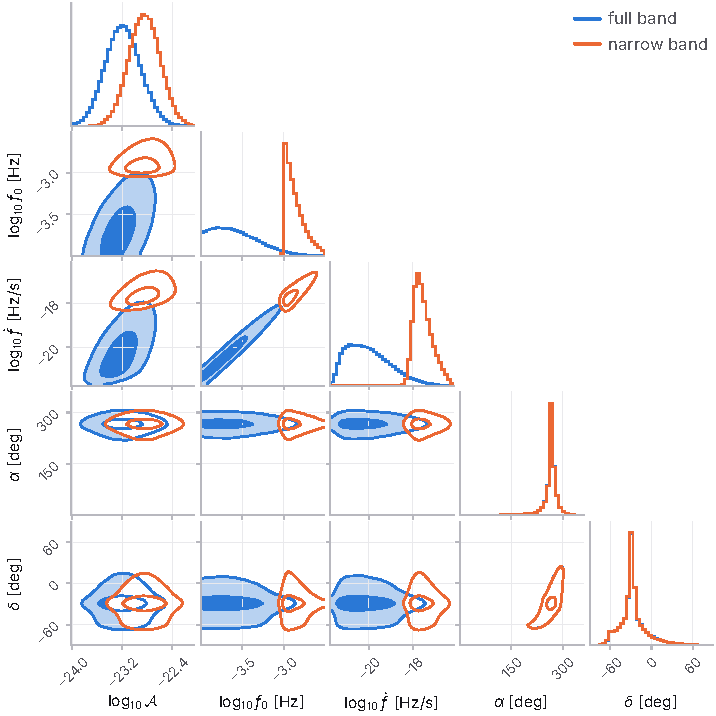
\includegraphics[width=0.62\textwidth]{figures/prior-corner.pdf}
  \caption{The per-source prior over each band (\cref{eq:priors-source,eq:priors-conditional,eq:priors-sky}):
  amplitude, frequency and drift in $\log_{10}$, and the equatorial sky $(\alpha, \delta)$, from
  \num{\PriorCornerDraws} draws per band with $f_0$ truncated to the band. Contours enclose
  \qty{\PriorCornerInner}{\percent} and \qty{\PriorCornerOuter}{\percent} of the draws (one and two standard deviations in two
  dimensions); diagonals are normalised marginals. The sky is drawn independently of the band, so its
  panels coincide; it is concentrated toward the galactic centre at
  (\ang{\PriorsCentreRa}, \ang{\PriorsCentreDec}) and along the plane.}
  \label{fig:prior-corner}
\end{figure*}
% updated 2026-11-09: was "S=\PriorsSources sources" (S = 4); the runs use S = 2 to 16.

\begin{table}[t]
\caption{Prior of one source $\theta = (f_0, \fdot, \Amp, \alpha, \delta, \psi, \iota, \phi_0)$ in
window $w$.}
\label{tab:priors-source}
\centering
\footnotesize
\begin{tabular}{@{}lp{0.68\columnwidth}@{}}
\toprule
parameter & prior \\
\midrule
$(f_0, \fdot, \Amp)$ & catalogue Gaussian in their logarithms, \cref{eq:priors-source} \\
\quad $f_0$ & its marginal, truncated to the window's interior, \cref{eq:priors-interior} \\
\quad $(\fdot, \Amp)\mid f_0$ & its conditional, \cref{eq:priors-conditional}, on $(0, \infty)^2$, uncut \\
$(\alpha, \delta)$ & bulge, two discs and a floor in galactic $(l, \sin b)$, \cref{eq:priors-sky} \\
$\psi$ & $\Unif(0, 2\pi)$ \\
$\iota\in[0,\pi]$ & $\cos\iota\sim\Unif(-1, 1)$ \\
$\phi_0$ & $\Unif(0, 2\pi)$ \\
\bottomrule
\end{tabular}
\end{table}

\begin{figure*}[t]
  \centering
  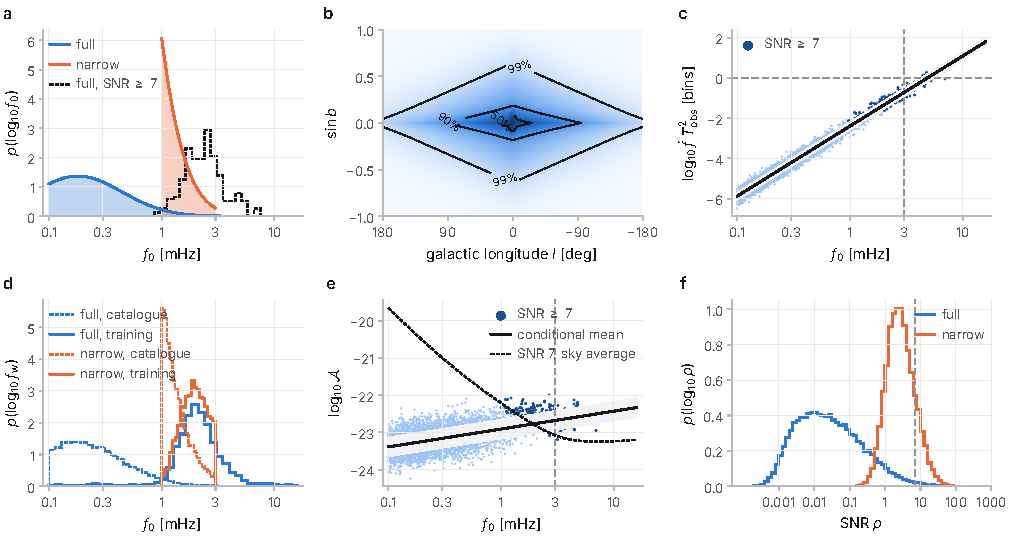
\includegraphics[width=\textwidth]{figures/priors.pdf}
  \caption{The prior over a window; lines are closed forms, filled steps and dots are
  \num{\PriorsPriorWindows} windows per band centred on the catalogue's $f_0$ marginal. (a)~$\log_{10}f_0$ of the drawn
  sources (filled) against the catalogue marginal truncated to each band (lines), and of the
  full band's visible sources, $\snr\ge\PriorsVisibleSnr$ (dashed). (b)~Sky, \cref{eq:priors-sky}, in the
  equal-area galactic $(l, \sin b)$: shading is the log density per steradian, contours enclose
  the marked share of the sources. (c)~Chirp drift over the observation, in frequency bins, in
  the full band: a sample of the sources (light), every visible one (dark), and the conditional
  mean of \cref{eq:priors-conditional} with its $\pm1\sigma$ residual (grey). Dashed: the narrow
  band's top and one bin. (d)~Where the window centres fall: on the catalogue's
  $f_0$ marginal (dashed) and by \cref{eq:priors-window} as in training (solid), per band. (e)~Amplitude, as in (c); dashed is the amplitude at which a
  source of mean-square sky and orientation reaches $\snr=\PriorsVisibleSnr$. (f)~\ac{snr} of each
  source alone in its window, per band; dashed at $\snr=\PriorsVisibleSnr$.}
  \label{fig:priors}
\end{figure*}

\subsection{Rates}
\label{sec:gw-rates}
% Formula moved 2026-11-10 from app:priors, "How many sources a window holds" (inline there).

Most sources lie far below the noise: in the
full band \qty{\RelatedWorkVisibleShare}{\percent} of them reach $\snr\ge\RelatedWorkSnrLow$
(\cref{app:priors}), with $\snr$ the signal-to-noise ratio of a source alone in its window
(\cref{sec:gw-waveforms}). The simulated Galaxy holds $N = \num{\RatesCatalogue}$ double white dwarfs
in the band. A window of $w$ bins centred at $f$ holds each with the probability $p(f,w)$ that its
$f_0$ falls in it under the catalogue's marginal $\pi(f_0)$, so it holds $n$ sources, $n_{\rm vis}$ of
them visible,
\begin{equation}
\begin{gathered}
  n \sim \operatorname{Bin}\bigl(N, p\bigr),\qquad n_{\rm vis} \sim \operatorname{Bin}\bigl(N, p_{\rm vis}\bigr),\\
  p = \textstyle\int_w \pi(f_0)\,\dd f_0,\qquad p_{\rm vis} = \textstyle\int_w \pi(f_0)\,P_{\rm vis}(f_0)\,\dd f_0,
\end{gathered}
  \label{eq:gw-rates}
\end{equation}
with $\int_w$ over the window and $P_{\rm vis}(f_0) = P\bigl(\snr\ge\RatesVisibleSnr\mid f_0\bigr)$,
the amplitude integrated out given $f_0$ (\cref{eq:priors-conditional}). A narrow-band window of
\RatesNarrowWindow{} bins holds on average \numrange{\RatesNarrowAllLo}{\RatesNarrowAllHi} sources and
\numrange{\RatesNarrowVisibleLo}{\RatesNarrowVisibleMax} visible ones, a full-band window of
\RatesFullWindow{} bins up to \num{\RatesFullAllHi} and \RatesFullVisibleMax{} (\cref{app:priors}).
Our $S\le16$ slots test how a joint posterior scales with $S$; a real analysis infers the number of
sources with a trans-dimensional sampler \citep{littenberg2020global} and models the rest as
confusion noise \citep{karnesis2021characterization}.

\subsection{Waveforms}
\label{sec:gw-data}\label{sec:gw-waveforms}
% Equations and figure moved 2026-11-10 from app:forward-model and app:noise (the details stay there).

A \ac{gb} emits a quasi-monochromatic wave at twice its orbital frequency that drifts slowly
through radiation reaction \citep{nelemans2001gravitational,korol2017prospects}. Its
transverse-traceless strain at the observer is
\begin{equation}
  h_{ij}(\xi) = h_+(\xi)\,e^+_{ij} + h_\times(\xi)\,e^\times_{ij},\qquad
  \xi = t - \frac{\hat{\mathbf k}\cdot\mathbf x(t)}{c},
  \label{eq:forward-model-xi}
\end{equation}
with $\hat{\mathbf k}$ the direction of propagation, set by $(\alpha,\delta)$, $\mathbf x(t)$ the
observer's position, $c$ the speed of light and $e^{+,\times}_{ij}$ the polarisation tensors of
the source frame, rotated by $\psi$ about $\hat{\mathbf k}$ (\cref{app:forward-model-waveform}). For a
circular binary with a constant frequency derivative,
\begin{equation}
\begin{aligned}
  h_+(\xi) &= -\Amp\,\bigl(1+\cos^2\iota\bigr)\cos\Psi(\xi),\\
  h_\times(\xi) &= -2\Amp\cos\iota\,\sin\Psi(\xi),\\
  \Psi(\xi) &= -\phi_0 + 2\pi f_0\,\xi + \pi\fdot\,\xi^2,
\end{aligned}
  \label{eq:forward-model-waveform}
\end{equation}
with every parameter at the start of the observation. Radiation reaction alone would fix the
drift by the chirp mass $\Mc$, with $G$ Newton's constant,
\begin{equation}
  \fdot = \frac{96}{5}\,\pi^{8/3}\left(\frac{G\Mc}{c^3}\right)^{5/3} f_0^{11/3};
  \label{eq:forward-model-fdot}
\end{equation}
the simulator keeps $\fdot$ free, with the prior of \cref{eq:priors-conditional}.
Over $\Tobs=\qty{\ForwardModelTobsYears}{\year}$ the
constellation's orbit modulates a source in amplitude and Doppler-shifts it, so in the frequency
domain it occupies a few bins to a few hundred around $f_0$. We simulate the link responses
\citep{finn2009response,cornish2009alternative} with the heterodyned fast response
\citep{cornish2007tests,jaxgb} on equal, constant arms \citep{lisaorbits}, form the \ac{tdi}~1.5
Michelson combinations $X$, $Y$, $Z$ \citep{tinto2021time} and from them the noise-orthogonal
channels \citep{prince2002lisa}
\begin{equation}
  A = \frac{Z-X}{\sqrt2},\quad E = \frac{X-2Y+Z}{\sqrt6},\quad T = \frac{X+Y+Z}{\sqrt3}.
  \label{eq:forward-model-aet}
\end{equation}
The noise is the instrument noise of the \ac{lisa} science requirements
\citep{lisasst2018lisa,babak2021lisa}: stationary, Gaussian, with one-sided \ac{psd} $S_c(f)$ in
channel $c$ (\cref{fig:noise-psd}a). On the window's Fourier bins $f_k$ (\cref{sec:gw-windows}),
with $\tilde h_c(f;\theta_s)$ the Fourier transform of source $s$'s response in channel $c$, the data
are
\begin{equation}
\begin{aligned}
  \tilde d_{k,c} &= \sum_{s=1}^{S}\tilde h_c(f_k;\theta_s) + \tilde n_{k,c},\\
  \tilde n_{k,c} &\sim \CN\!\bigl(0,\ P_c(f_k)\bigr),\qquad
  P_c(f) = \tfrac12\,S_c(f)\,\Tobs,
\end{aligned}
  \label{eq:noise-data}
\end{equation}
with $\CN$ the circular complex Gaussian, independent across bins and channels. With the noise-weighted inner product
\citep{cutler1994gravitational}
\begin{equation}
\begin{aligned}
  \inner{a}{b} &= 4\,\mathrm{Re}\sum_{c}\sum_{k}\frac{a_{k,c}\,b^*_{k,c}}{S_c(f_k)\,\Tobs}\\
  &= 2\,\mathrm{Re}\sum_{c}\sum_{k}\frac{a_{k,c}\,b^*_{k,c}}{P_c(f_k)},
\end{aligned}
  \label{eq:inner}
\end{equation}
the log-likelihood of a window is the Whittle likelihood of \cref{eq:noise-data},
\begin{equation}
\begin{aligned}
  \log p(d\mid\theta_{1:S}) &= -\tfrac12\inner{d-h}{d-h} + \text{const}\\
  &= -\sum_{k,c}\frac{\bigl|\tilde d_{k,c}-\tilde h_{k,c}(\theta_{1:S})\bigr|^2}{P_c(f_k)} + \text{const},\\
  \tilde h_{k,c}(\theta_{1:S}) &= \sum_{s}\tilde h_c(f_k;\theta_s).
\end{aligned}
  \label{eq:loglik}
\end{equation}
and a source's signal-to-noise ratio $\snr_s$ is given by $\snr_s^2 = \inner{h(\theta_s)}{h(\theta_s)}$
(\cref{app:noise-snr}). The network sees the data whitened by $P_c$ (\cref{app:noise}).
% updated 2026-11-09 (moving the definition of theta to the section's head): "modulates it" -> "modulates a source".

\begin{figure*}[t]
  \centering
  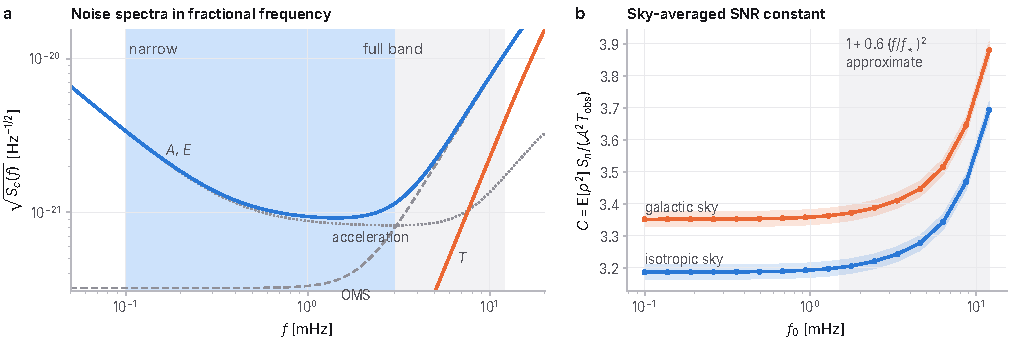
\includegraphics[width=\textwidth]{figures/noise.pdf}
  \caption{The noise and the amplitude unit built on it. (a) Amplitude spectral densities
    $\sqrt{S_c}$ of \cref{eq:noise-psd}, with the \acs{oms} and acceleration terms of $S_A$
    alone: acceleration noise dominates below a few \unit{\milli\hertz}, and $T$ is orders of
    magnitude quieter there. Shading marks the narrow and full bands. (b) The sky-averaged
    constant $C$ of \cref{app:noise-snr}, measured with our \acs{snr} for an isotropic and a
    Galactic sky ($\pm$ one standard error): flat at low frequency, rising at the top of the full
    band, where $1+0.6(f/f_\star)^2$ only approximates the response.}
  \label{fig:noise-psd}
\end{figure*}

\subsection{Frequency-Domain Factorisation}
\label{sec:gw-factorisation}

\textcolor{red}{TODO(move from \cref{app:forward-model-windows}): why the likelihood of the band
factorises into windows.}

\subsection{Slicing in Frequency}
\label{sec:gw-windows}

The observation $y$ is a window of $K$ whitened bins in each channel,
$K\times6$ real numbers, centred at $\fw$.
We train two configurations (\cref{tab:forward-model-bands}): the narrow band, windows of
\PriorsNarrowW{} bins with \qtyrange{\PriorsNarrowLowMhz}{\PriorsNarrowHighMhz}{\milli\hertz}, where sources
crowd the most; and the full band, windows of \PriorsFullW{} bins up to
\qty{\PriorsFullHighMhz}{\milli\hertz}, where a source's drift and Doppler spread cover up to
a hundred bins.
% updated 2026-11-09: the narrow band was "f0 <= \PriorsNarrowHighMhz mHz"; it now starts at 1 mHz.

\subsection{Tokenisation}
\label{sec:gw-tokens}

The data stream of the network (\cref{sec:method-network}) reads the window as
a short-time Fourier transform, \NetworkPatch{} bins per token, each token holding its band's time
samples in the three channels (\cref{eq:network-stft}): \NetworkTokensNarrow{} tokens in the
narrow band, \NetworkTokensFull{} in the full band.
% updated 2026-11-09 (moved out of the Network subsection): "The data stream" -> "The data stream of
% the network (sec:method-network)".
